\documentclass[12pt]{article}

\usepackage{times}
\usepackage{notes}
\usepackage{url}
\usepackage{graphicx}

\setlength{\textwidth}{6.5in}
\setlength{\textheight}{8.9in}
\setlength{\oddsidemargin}{0.0in}
\setlength{\topmargin}{0.05in}
\setlength{\headheight}{-0.05in}
\setlength{\headsep}{0.0in}

\begin{document}

\begin{center}
  {\bf CS 6300} \hfill {\large\bf HW03: Expectimax and Probability} \hfill {\bf Due February 6, 2023}
\end{center}

Please use \LaTeX\ to produce your writeups. See the Homework
Assignments page on the class website for details.

\section{Expectimax}

Consider the zero-sum expectimax game tree below.  Circles represent
chance nodes.  Trapezoids that point up represent choices for the
player seeking to maximize. Outcome values for the maximizing player
are listed for each leaf node.

\begin{enumerate}

\item First, assume that each chance node chooses uniformly between
  available moves. Assuming optimal play, carry out the expectimax
  search algorithm and write the value of each node inside the
  corresponding trapezoid. What is the expected value of this game
  assuming optimal play? What is the optimal move to make at each
  node?  Fill in the node values using a drawing program.

\begin{center}
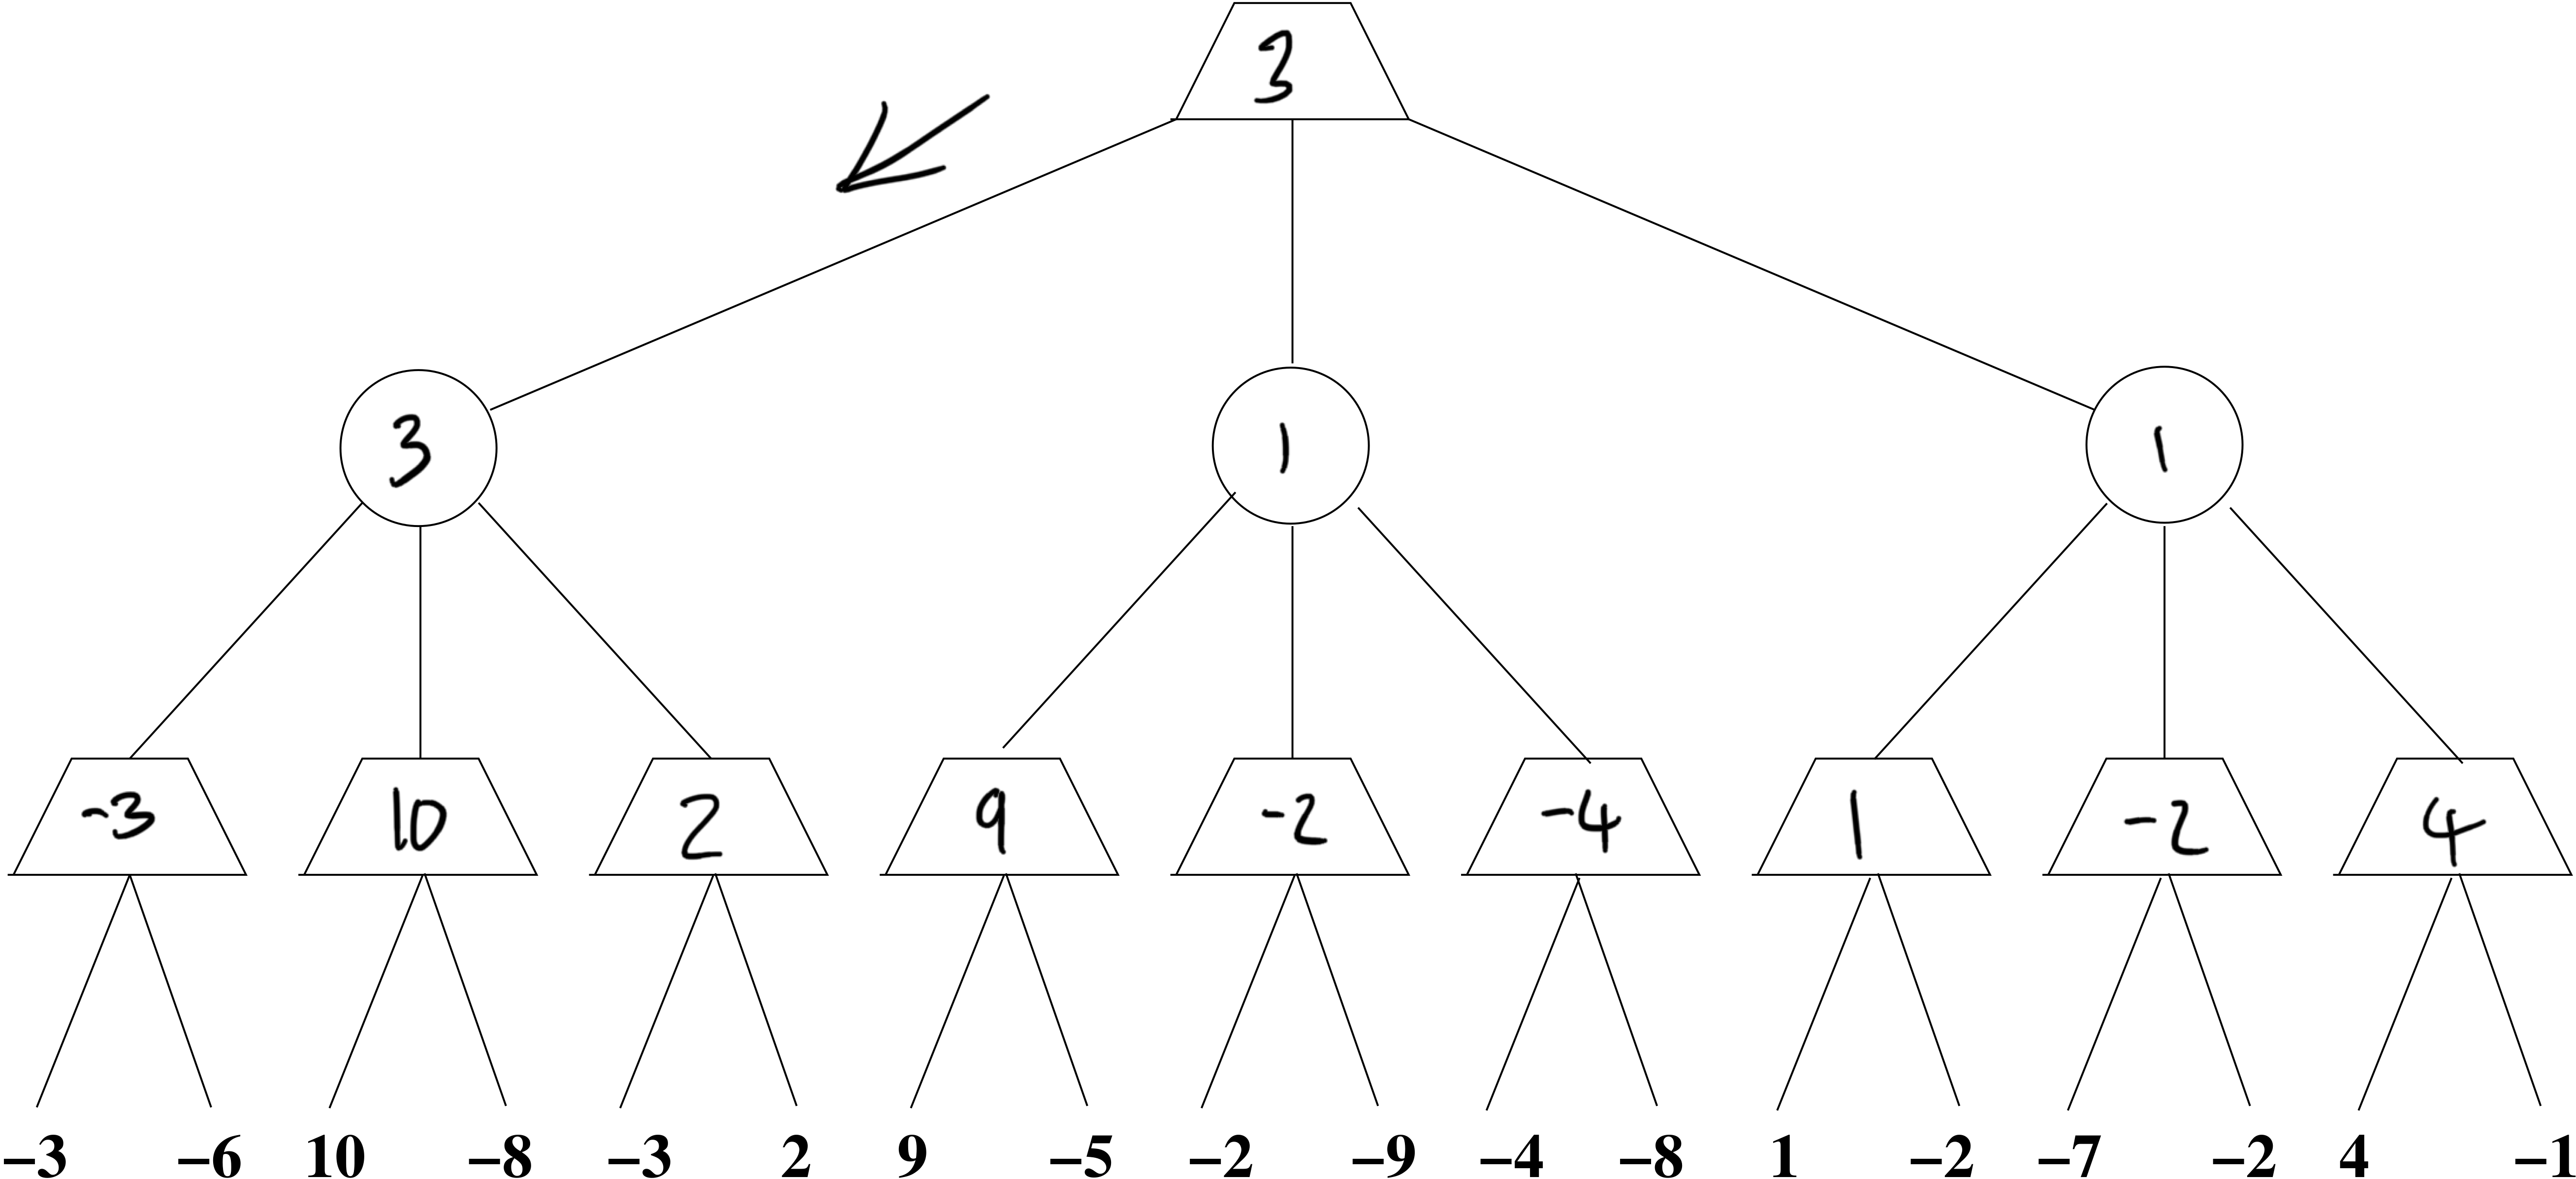
\includegraphics[width=6in]{Q1.png}
\end{center}

Moving left is the optimal move leading to an expected game value of 3.

\clearpage

\item Now, assume that each chance node plays the leftmost move with
  probability 0.5, the middle move with probability 0.25, and the
  rightmost move with probability 0.25. Assuming optimal play, what is
  the expected value of this game?  What is the optimal move to make?
  Fill in the node values using a drawing program.

\begin{center}
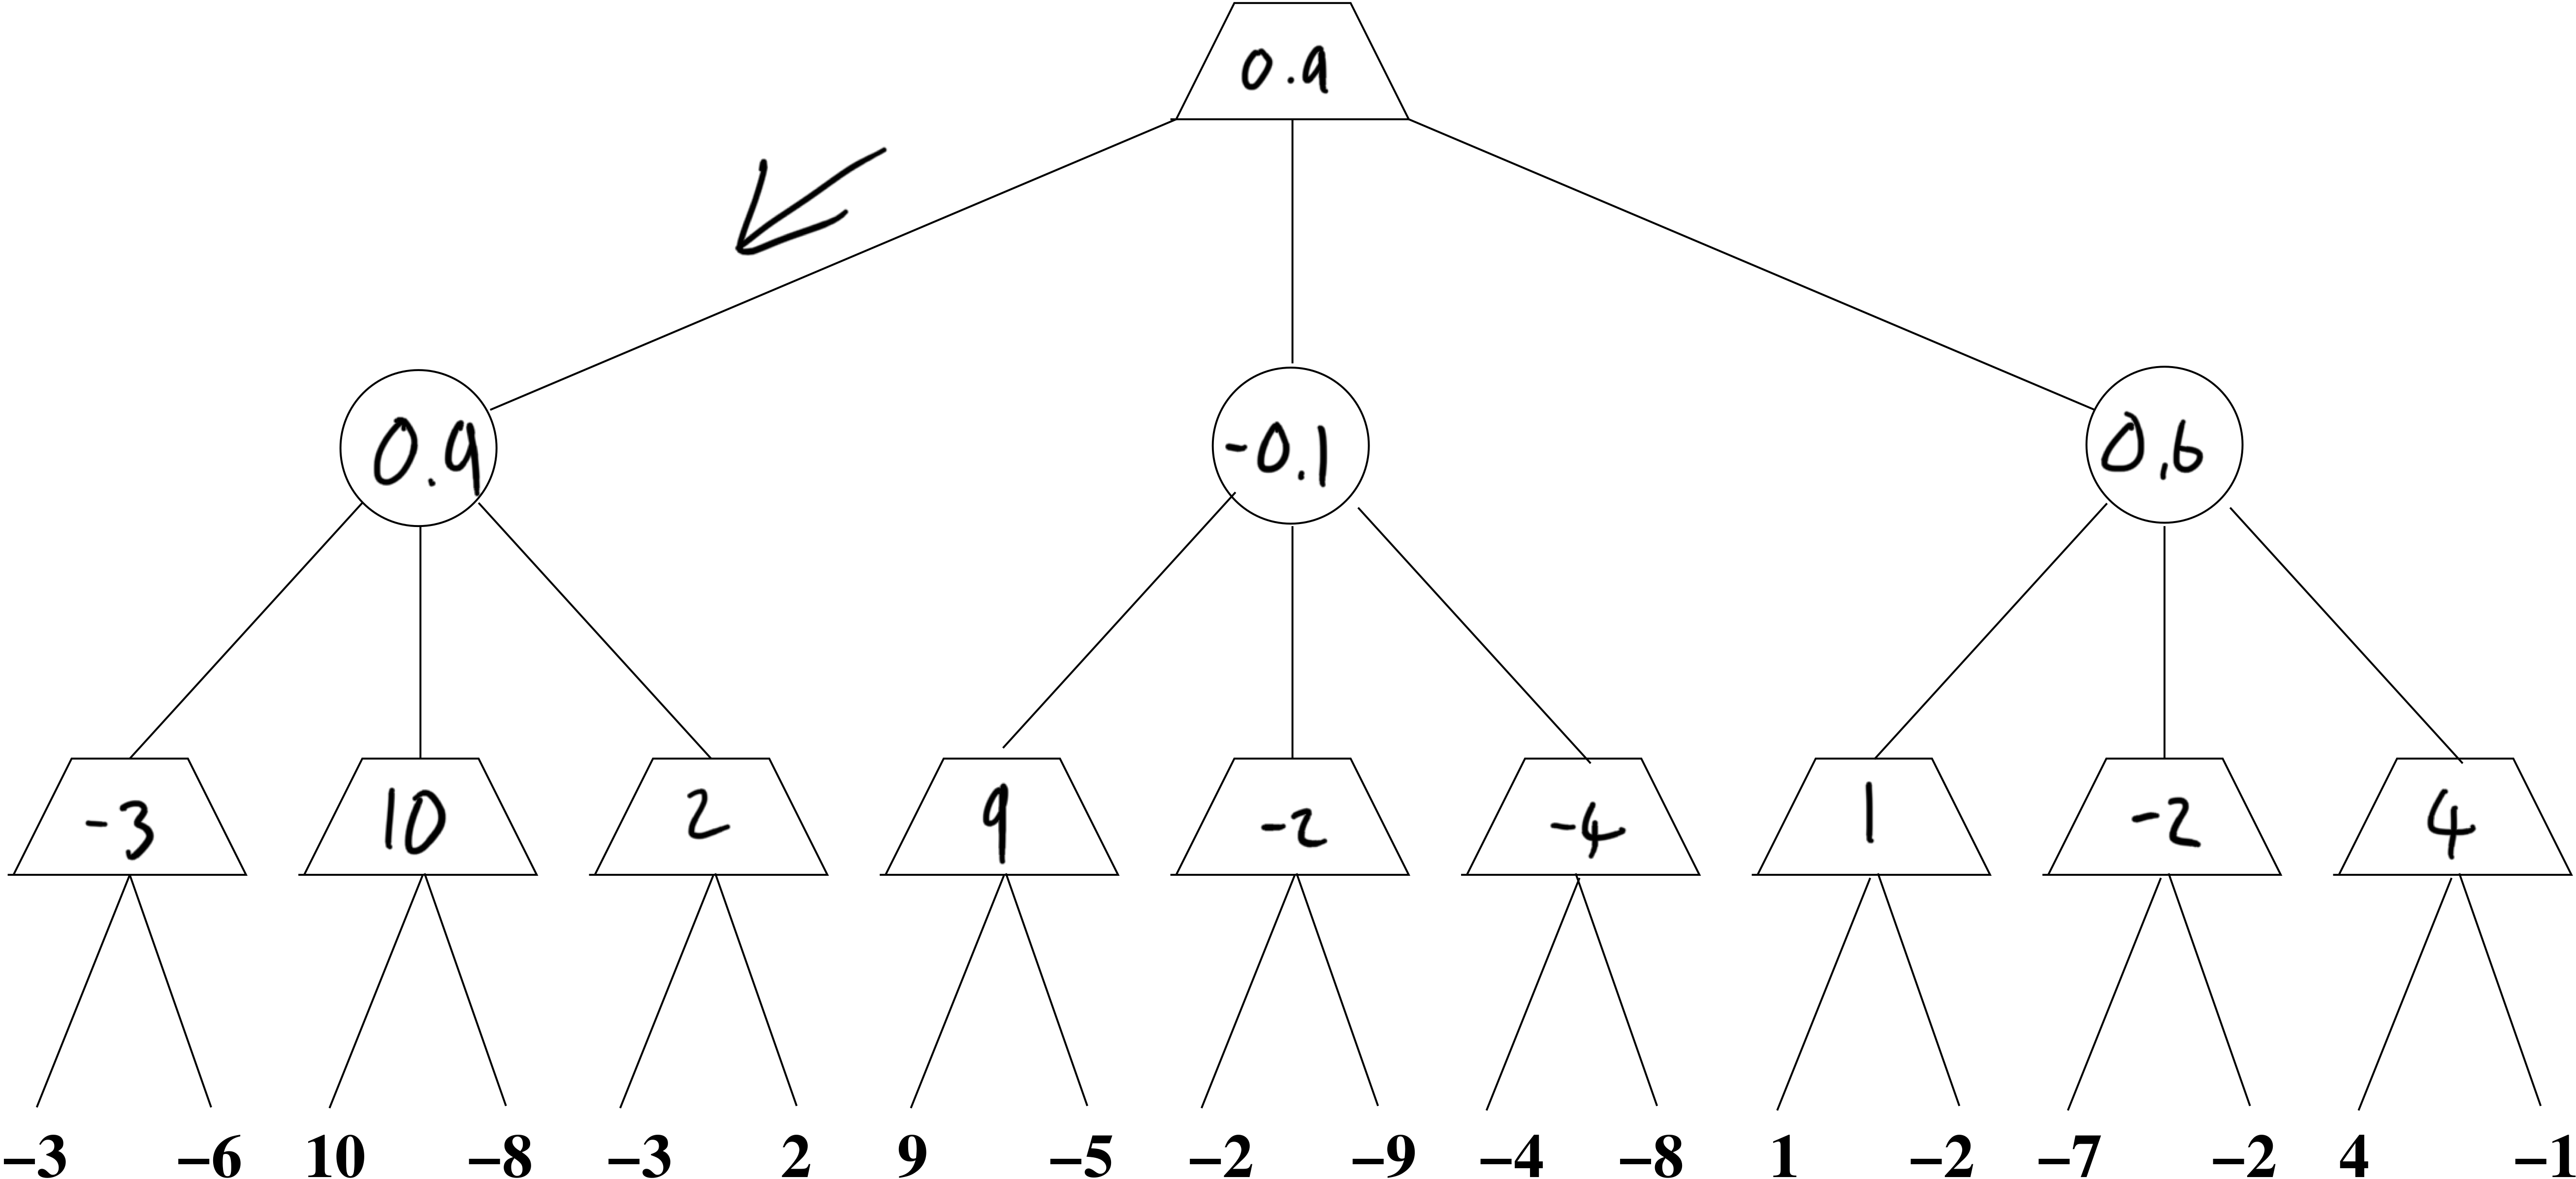
\includegraphics[width=6in]{Q2.png}
\end{center}

Moving left is the optimal move leading to an expected game value of 0.9.

\end{enumerate}

\clearpage

\section{Probability}

Consider the following probability tables for variables $A,B,C$.

\begin{center}
\begin{tabular}{ccc}
\begin{tabular}{|r|r|} \hline
A  & $P(A)$ \\ \hline
+a & 0.3      \\ \hline
-a & 0.7      \\ \hline
\end{tabular} &
\begin{tabular}{|r|r|r|} \hline
B  & A  & $P(B|A)$ \\ \hline
+b & +a & 0.7      \\ \hline
+b & -a & 0.6      \\ \hline
\end{tabular} & 
\begin{tabular}{|r|r|r|} \hline
C  & A  & $P(C|A)$ \\ \hline
+c & +a & 0.2      \\ \hline
+c & -a & 0.9      \\ \hline
\end{tabular}
\end{tabular}
\end{center}

\begin{enumerate}

\item Derive $P(A,B)$ by filling in the entries below.  What formula are you using?

\begin{center}
\begin{tabular}{|r|r|r|} \hline
A  & B  & $P(A,B)$ \\ \hline
+a & +b &  0.21        \\ \hline
+a & -b &  0.09        \\ \hline
-a & +b &  0.42        \\ \hline
-a & -b &  0.28        \\ \hline
\end{tabular}
\end{center}

I'm using the product rule, $P(A,B) = P(A) \times P(B|A)$

\item Derive $P(A|C)$ by filling in the entries below.  What formula are you using?

\begin{center}
\begin{tabular}{|r|r|r|} \hline
A  & C  & $P(A|C)$ \\ \hline
+a & +c & 0.087         \\ \hline
+a & -c & 0.774         \\ \hline
-a & +c & 0.913         \\ \hline
-a & -c & 0.226         \\ \hline
\end{tabular}
\end{center}

I'm using Bayes' formula to find the reverse of $P(C|A)$ as per the lecture

\item Suppose $B$ and $C$ are conditionally independent given $A$.
  What is the formula you would use?  Then derive the full joint
  distribution $P(A,B,C)$ by filling in the entries below.

\begin{center}
\begin{tabular}{|r|r|r|r|l|l|} \hline
A  & B  & C  & $P(A,B,C)$ \\ \hline
+a & +b & +c & 0.042           \\ \hline
+a & +b & -c & 0.168           \\ \hline
+a & -b & +c & 0.018           \\ \hline
+a & -b & -c & 0.072           \\ \hline
-a & +b & +c & 0.378           \\ \hline
-a & +b & -c & 0.042           \\ \hline
-a & -b & +c & 0.252           \\ \hline
-a & -b & -c & 0.028           \\ \hline
\end{tabular}
\end{center}

I'm using $P(A,B,C) = P(A) \times P(B|A) \times P(C|A)$

\item Derive the conditional distribution $P(A|+b,-c)$.  What formula
  would you use?  Then fill in the table below.

\begin{center}
\begin{tabular}{|r|r|r|r|l|l|} \hline
A  & B  & C  & $P(A|+b,-c)$ \\ \hline
+a & +b & -c & 0.8             \\ \hline
-a & +b & -c & 0.2             \\ \hline
\end{tabular}
\end{center}

I'm looking at the rows above that have $+b, -c$ and finding the probability of $A$

\end{enumerate}

\end{document}
